% !TEX root = _main.tex

% ==========================================
% ここから本文．あとは各自で
% ==========================================

% １章と２章
% !TEX root = _main.tex
%1
\section{はじめに}

近年インターネットの普及に伴い音楽の楽しみ方が大きく変化している．
従来ではCDを購入してプレイヤーで楽しむことが一般的であったが，近年はインターネット配信で楽しむ人が増加している．
各音楽配信サイトなどでは，ユーザの嗜好に合った楽曲の検索を容易にするために楽曲を音楽ジャンル別で分類されることが多くみられる．

音楽ジャンル解析は古くから数多くの研究が行われており，近年では主要な研究テーマの１つとして扱われている．
しかし，楽曲のジャンルは時系列で変わっていくのではないだろうか？
%
\red{例えば，}Mrs. GREEN APPLEの「ライラック」\cite{lilac}%があげられる．
%この楽曲
\red{で}は，冒頭約10秒間でギターにエフェクトを加えた電子音が流れる．
しかし，その後同じフレーズをドラムやギターの音色で構成する．
これにより，電子音のような音色では感じることのなかったロックミュージックの印象を抱かせるものとなっている．
このように，聴取する箇所によって抱く印象が異なる楽曲が存在すると考える．

%しかし，これらの大半は１つの楽曲を1つの音楽ジャンルに分類するものである．
%このような音楽ジャンルの分類方法では，楽曲内における音楽ジャンルの変化の識別が困難であると考える．

そこで本研究では，数ある音響特徴量の中でも\red{音色に着目し，対象楽曲の楽器構成から\footnotemark}音楽ジャンルの変化を時系列で表示するシステムを提案することを目的とする．
\footnotetext{\red{「音色」に着目して（いろいろ検討した結果，）楽器構成を手掛かりにジャンル分析をするのがよいとした，その思考プロセスを２章でしっかり語るべし．}}



%2
\section{先行研究}
現在まで，音楽ジャンル解析に関する研究は数多く行われている．楽曲のパート編成やピッチ，音長，リズムパターン，音色，リズム特性などといった特徴量を対象とした研究がある\red{（［文献URL追加］）}．
\red{ジャンル推定をするのに，なぜ楽器編成に着目するのか？従来研究の知見とともにりささんの主張をここで言う．}


\subsection{\red{楽器構成に着目したジャンル推定}}


土橋らは音響信号の中でもベースパートに着目し，ベースパートの特徴量，音色，リズムを用いた音楽ジャンル推定を行っている\cite{bassline}．また，鈴木らは旋律パートのみを用いて音楽ジャンル判別を行うための新たな特徴量を提案し，その有効性を検証している\cite{melody}．

Basiliら\cite{basili}はMIDIデータから楽曲のパート編成やピッチ，音長といった高次の特徴量を抽出し，機械学習アルゴリズムを用いて音楽ジャンルを分類している．

また，楽器構成の抽出を応用した研究も行われている．

卓見ら\cite{takumi}らは，楽器編成を自動認識し，それを用いて楽曲を探索するための手法を開発している．
楽器編成の認識方法には畳み込みニューラルネットワーク（CNN）を使用し，既存の方法よりも高精度な認識が達成された．

Yoonchang Hanら\cite{han}は，畳み込みニューラルネットワーク（ConvNet）を使用して，ポリフォニック音楽の音源から主要楽器を識別する方法を提案している．
なお，ポリフォニック音楽とは複数の楽器が同時に演奏される音楽である．
畳み込み層とプーリング層を繰り返し使用したConvNetを採用し，結果として，ConvNetは精度と再現率において従来の手法を上回っている．


\subsection{\red{時系列の推移に対応した類似演奏の探索}}
\red{
	query-by-conducting，mazurka projectみたいなことをしたい．という話がごっそりぬけている．
	図を引用してきていいので，自分が「時系列に対応したジャンル推定」の出力がどういうイメージを持っているのかを示す．
	音楽の類似度（music similarity）をどうやって計算するか，という話も本当はしたい．
	少なくとも質問されたら答えられるように！
}

\subsection{\red{本研究の狙い}}
\red{
	本研究が目指す世界（達成したいこと）が何かを明確にする．
	ポイントは，(1)楽器編成に注目するとジャンル分析がうまくいく（という期待があること）
	(2) 時系列で区切って，区間別にジャンルっぽさの変化の様子を可視化したい
}

上記で記した研究は１つの楽曲に対して１つのジャンルを判別するものであり，従来はこの判別方法が典型であった．しかし，本研究では楽曲を時間で区切ることにより，楽曲内の音楽ジャンルの変化を可視化することが可能となる．



\section{研究概要}
\figref{fig:system}に，提案システムのシステムの処理の流れを示す．

\begin{figure}[tb]
	\centering
	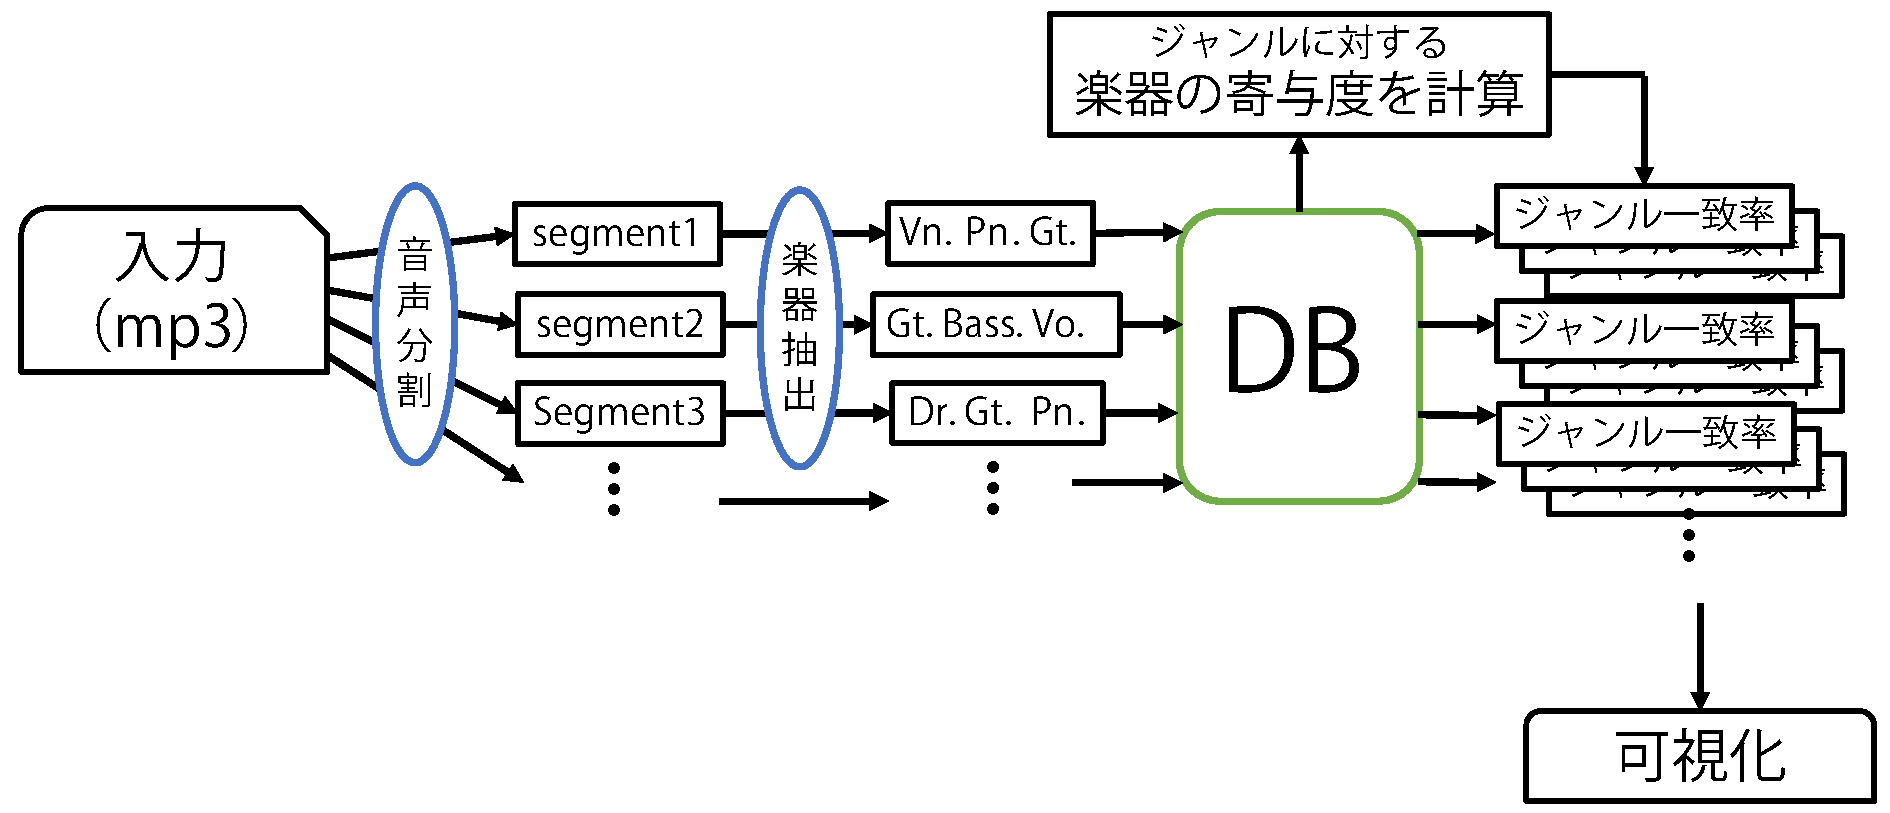
\includegraphics[width=\hsize]{fig/fig18-system.pdf}
	\caption{処理の流れ}
	\label{fig:system}
\end{figure}

%分析する楽曲を対象楽曲とし，対象楽曲の
入力は，MP3形式の音響信号とする．
入力音声に対し，機械学習モデルを用いて楽器構成を抽出する．次に，抽出された楽器構成に対してデータベースとの照合を行い，ジャンルの一致率を算出する．
分析結果はグラフとして視覚化し，ジャンルの変化と優勢性を示す．

%提案システムの構成は主に音色の抽出，音楽ジャンルの解析，計算結果の表示の３つにわけることが出来る．
%データベースと入力データの前処理について記述した後，システムの詳細を記述する．

\subsection{楽曲データベース}
音楽ジャンル分析には，独自に収集したデータセットを使用する．
jazz，classic，rockの３ジャンルを対象とし，各ジャンル50曲，合計150曲の楽曲を選定した．
対象とした３ジャンルは特定の楽器を使用することが多く，本研究に適切であると考えたために選出した．
使用楽曲は，音楽配信サービスSpotify\cite{spotify}にて各ジャンルの名盤を検索し，人気順で選定した．
また，正確なジャンル分類を保証するため，Apple MusicおよびAmazon Musicのジャンル情報とも一致する楽曲のみを選定した．

収録する楽曲情報は楽曲名，音楽ジャンル，楽器構成である．

Spotifyを主なデータソースとし，スコアや楽曲クレジット情報を元に使用されている楽器構成を抽出した．
一部の楽曲についてスコア（総譜）や詳細な楽曲クレジット情報が不足している場合には，聴取による推定や補足を行った．
ソフトウェア音源を使用して楽器の音色を再現している楽曲については，再現している楽器として抽出した．
また，エフェクトがかかっており元の楽器の音色が判別できない音や，コンピュータで作成された音源のため楽器の音と判別できない音がある．
これらの楽器は一律に電子音（シンセサイザ）とした．

本システムで使用する楽器名を\tabref{tab:instrument}に示す．
対象とする楽器は、データベースの楽曲で使用されている楽器である。

\begin{table*}[tb]
	\centering
	\caption{システムで扱う楽器名の一覧}
	\scriptsize
	\begin{tabular}{c||c} \hline
		カテゴリ & 楽器名                                                                                \\ \hline\hline
		弦楽器  &
		\begin{tabular}{c}
			バイオリン，チェロ，ヴィオラ，コントラバス，ギター， \\ エレキギター，アコースティックギター，ベース，ハープ，マンドリン \\
		\end{tabular}                            \\ \hline
		木管楽器 &
		\begin{tabular}{c}
			フルート，ピッコロ，クラリネット，オーボエ， \\ ファゴット，サックス，トラヴェルソ，コーラングレ \\
		\end{tabular}                                        \\ \hline
		金管楽器 &
		\begin{tabular}{c}
			トランペット，コルネット，トロンボーン，バストロンボーン， \\ チューバ，ユーフォニアム，ホルン \\
		\end{tabular}                                         \\ \hline
		打楽器  &
		\begin{tabular}{c}
			ドラム，ティンパニ，シンバル，グロッケンシュピール，コンガ， \\ バスドラム，スネアドラム，タムタム，タンバリン，\\ シロフォン，ベル，マラカス，ウッドブロック，カスタネット \\
		\end{tabular} \\ \hline
		鍵盤楽器 & ピアノ，オルガン，ハープシコード                                                                   \\ \hline
		電子楽器 & キーボード，シンセサイザ                                                                       \\ \hline
		その他  & ボーカル，コーラス，電子音，ホイッスル                                                                \\ \hline
	\end{tabular}
	\label{tab:instrument}
\end{table*}

作成したデータベースの一部を\tabref{fig:database}に示す．

\begin{table}[tb]
	\centering
	\caption{データベース（一部のみ．詳細は付録\ref{app:database}を参照）}
	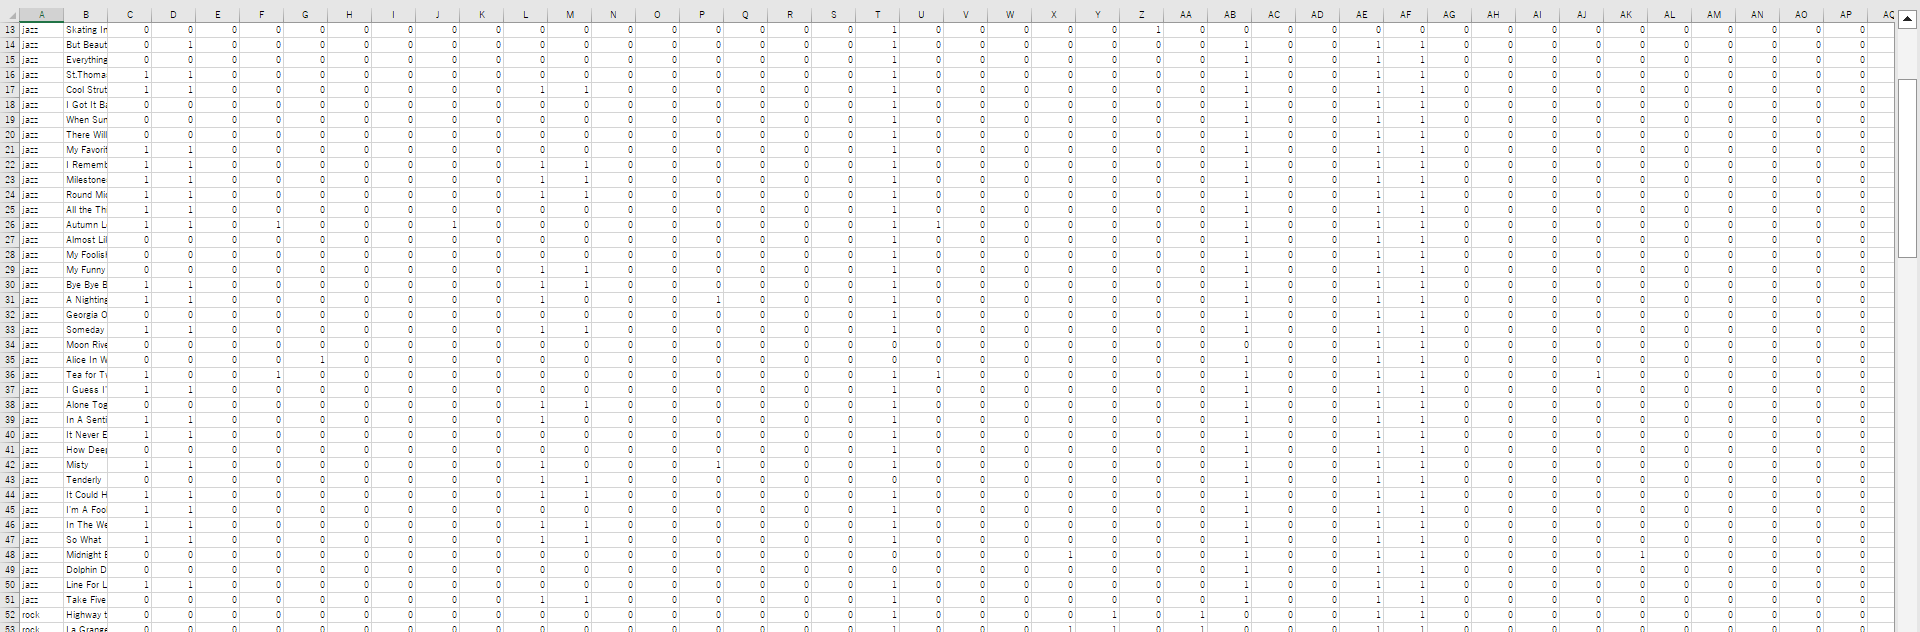
\includegraphics[width=\hsize]{fig/fig11-database.png}
	\label{fig:database}
\end{table}

%\subsection{音色の抽出}
%本研究では時間推移における楽器構成の変化を捉え，対象楽曲の楽器構成から音楽ジャンルの変化を分析する．
\subsection{楽器構成の抽出}
まず，入力音声ファイルを３秒ごとのセグメントに分割する．

データベースの楽曲において，楽器の変動が最も多い楽曲を分析した．
その結果，最も早く楽器構成が変化するのが３秒間であった．
また，分割秒数を短時間にすると楽器構成の抽出精度が低下した．
これらの理由から，分割秒数は３秒とした．

%音声ファイル名のフォルダを新たに作成し，作成フォルダ内に各セグメントを格納する．
%音声ファイル名のフォルダが既に存在する場合には，この処理は行わずに既存のセグメントを解析に用いる．
%これにより，データの重複を防ぐことが可能である．
%
次に，各セグメントに対し，楽器構成を抽出する．

楽器の抽出には，Pretrained Audio Neural Networks (以下PANNsと記述)\cite{PANNs} を活用し，畳み込みニューラルネットワーク（CNN）を基盤とするモデル Cnn14\_DecisionLevelMax を用いて楽器分類を行う．
PANNs とは，大規模データセットであるAudioSetで事前学習された音響イベント分類用のニューラルネットワークである．
CNNベースのアーキテクチャを持ち，音響特徴量を抽出し，分類や特徴量として利用できる．
Cnn14\_DecisionLevelMaxとは，PANNsの一種で，音響イベント分類のために設計されたCNNモデルである．
最大プーリング(Max Pooling)を採用して最も強い音響特徴量を反映することで，分類精度を向上させている．

対象とする入力音源はmp3ファイルである．楽器分類に適した形に前処理を施した後，モデルによる推論を行う．
その後，各楽器の確信度を計算しながら最終的な構成を決定する（\figref{fig:audio}）．

%以下具体的な処理内容について記述する．

入力された音声ファイルに行う前処理はリサンプリング、ノイズ除去、低周波・高周波フィルタの適用、正規化の４つである。

\begin{figure}[tb]
	\centering
	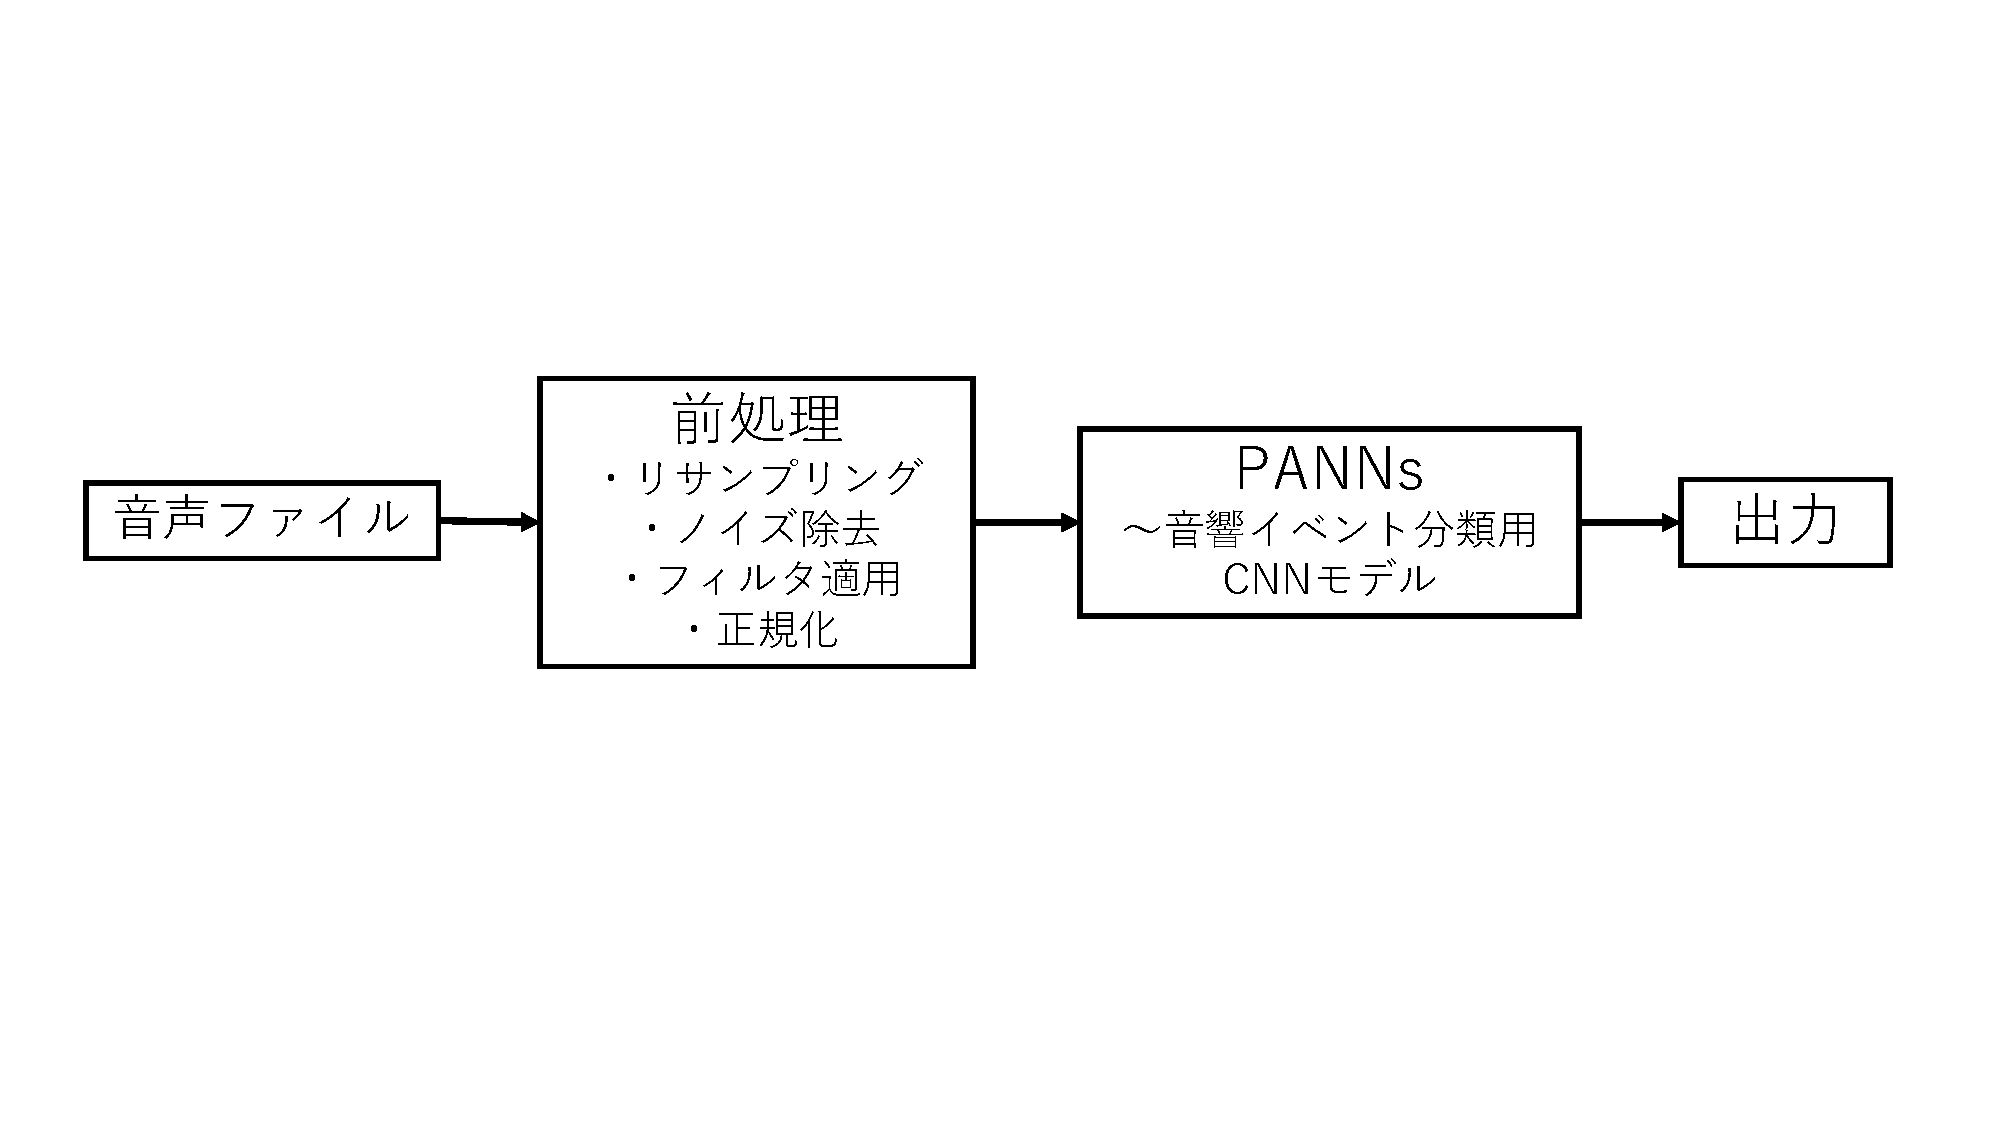
\includegraphics[width=\hsize]{fig/fig20-audio.pdf}
	\caption{楽器抽出の流れ}
	\label{fig:audio}
\end{figure}

PANNsは32kHzのサンプリングレートを前提として訓練されている．
そのため，入力音声を32kHzにリサンプリングする前処理を行う．
また，不要なノイズの低減と，高周波成分の協調，打楽器成分の分離のために，ノイズ除去および高周波・低周波フィルタの適用を行う．
高周波・低周波フィルタでは1000Hzから14000Hzの音のみを通すバンドパスフィルタを使用することで、打楽器とその他楽器の音の抽出が正確になる。
さらに，標準偏差に基づく正規化を行い，音量バランスを調整することで，音響特徴の抽出精度を向上させる．
これらの前処理により，不要な雑音や音量変化の影響を受けにくくなる．

上記の前処理後の音声データをPANNsに入力し，50回の反復推論を実施して結果の安定化を図る．
これにより，少ない反復推論では検出されなかった楽器が検出される．
この推論結果として，527クラスに分類された楽器・音響ラベルの確信度スコアが得られる．

この出力を基に，特定の楽器に対応するラベルを抽出し，あらかじめ設定したしきい値と比較することで，最終的な楽器構成を決定する．
しきい値はデータベースの音源をもとに，それぞれの分類結果に適したしきい値を設定した．

以上の処理によって抽出された楽器構成リストは，入力音声ファイルと同名のフォルダ内にテキストファイルとして保存される．
この楽器抽出方法は，精度の向上を図るために処理時間が長くなるという課題がある．
楽器構成リストをテキストファイルとして保存することで，二度目に音楽ジャンル推定を行う場合の楽器抽出処理が不要となる．
これにより，過去に音楽ジャンル推定を行った楽曲の処理時間を短縮することが出来る．

%これはISMIR 2023\cite{ISMIR2023}で発表されたもので，ものである．


% -----以下，どこにつながる話かわからない...のでコメントアウト ------
% 表２は，LP-MusicCapsの整合性を示したものである\red{（どれのこと？）}．
% 使用楽器数が少ない楽曲では高い整合性があることがわかる．
% しかし，楽器構成が複雑になるほど正確に抽出することが困難である傾向があると考える\red{（だから何？どこにつながる話？）}．


% 図２は音色の抽出手法のシステム構成図である\red{（どれのこと？）}．

% LP-MusicCapsは音声データからテキスト生成するテキストである．
% 音声ファイルをLP-MusicCapsの外部webサイトを介して生成されたテキストを取得する．
% ------ここまでコメントアウト------

% ------以下は４章（実装へ）に移動 ----------
% LP-MusicCapsで生成されたテキストはセグメントが保存されているフォルダ内にテキストファイルとして保存される．

% しかし，外部webサイトを介した処理を行う場合に処理速度が遅くなるという問題がある．
% 解決方法として，すでに入力音声ファイルと同名のフォルダが存在する場合にはLP-MusicCapsを介した処理を行わず，フォルダ内に存在するテキストファイルからテキストを取得する処理を追加した．
% これにより，過去に解析したことのある楽曲を再度解析する際の処理速度が短縮される．

%抽出されたテキストのうち，楽器名の記述部分のみを抽出し，当該セグメントの楽器構成としてリスト化する．

以上の処理をすべてのセグメントに対して行い，時間ごとの楽器構成を抽出する．

\subsection{音楽ジャンルの一致率分析}
本研究では，各ジャンルの中で対象楽曲がジャンルGである確率を，「ジャンルの一致率」と定義する．

抽出した楽器情報を用い，データベースと照合しながら各ジャンルに対する一致率を算出する．
具体的には，ジャンルごとの楽器出現頻度を用いた重み付けを行い，検出された楽器の出現確率を基にジャンルごとの確率を計算する．
この際，各楽器の出現頻度に対する対数変換を施すことで，対象楽器の寄与度を調整しつつ，一般的な楽器の影響を適切に反映するよう工夫した．

以下で計算式とともに計算手順を記述する．

\textbf{(１)楽器ごとの重み計算}

音楽ジャンルを識別するために有効な楽器は，特定のジャンルに特有の楽器である．
つまり，どのジャンルにも頻出する楽器ではなく，特定のジャンルでのみ頻出する楽器が音楽ジャンルの識別において重要である．
そこで，楽器の出現頻度に基づく重み付けを行うことで，各ジャンルに及ぼす楽器の影響を考慮する．

ジャンル$G$における楽器$i_k$の平均出現確率$P(i_k|G)$は，データセット内の楽曲における該当楽器の平均値として定義される．

\begin{equation}
	P(i_k | G) = \frac{1}{N_G} \sum_{j=1}^{N_G} x_{j, i_k}
\end{equation}

$x_{j, i_k}$は楽曲$j$における楽器$i_k$の有無，$N_G$はジャンル$G$に属する楽曲の総数である．

ジャンル$G$の重みは以下のように定義する．

\begin{equation}
	w_{i_k, G} = \log \left( \frac{N_G + 1}{\sum_{j=1}^{N_G} x_{j, i_k} + 1} \right)
\end{equation}

\textbf{(２)確率推定}

対象楽曲の楽器リスト$I$が与えられたとき，各ジャンル$G$での事後確率$P(I|G)$を以下のように求める．

\begin{equation}
	P(I|G) \propto \prod_{i_k \in I} P(i_k | G)^{w_{i_k, G}}
\end{equation}

各楽器の確率に対して重み$w_{i_k, G}$を指数として乗算することで，楽器の重要度が考慮される．
さらに，ゼロ除算を防ぐために各確率値には小さい平滑化パラメータ\( \epsilon \)を適用する．

\begin{equation}
	P(i_k | G) = \max (P(i_k | G), \epsilon), \quad \epsilon = 10^{-6}
\end{equation}

\textbf{(３)正規化}

上記の計算により，各ジャンルの未正規化確率 \( P(I|G) \) が求まる．
最終的な確率分布を得るために，すべてのジャンルの確率を合計し，正規化する．

\begin{equation}
	P'(G|I) = \frac{P(I|G)}{\sum_{G'} P(I|G')}
\end{equation}

$P'(G|I)$は最大値を1.0として，数値が大きいほど一致度が高いことを示す．
$P'(G|I)$をパーセント表記に変換し，小数点以下２桁までで表示する．

\begin{equation}
	P_{\text{percent}}(G|I) = \lfloor P'(G|I) \times 100 \rfloor / 100
\end{equation}

上記の処理をセグメントごとに各ジャンルに対して行う．

さらに，与えられたジャンル一致率をもとに，時間セグメントごとにジャンルの一致率を視覚化する．
本システムでは，各セグメントにおけるジャンル確率の分布を比較し，一致率の高いジャンルを特定するために棒グラフを用いた．
各セグメントごとのジャンル確率を棒グラフとして表示し，音楽ジャンルごとに色分けをした．
これにより，ジャンルの優勢性を明確に示すよう設計している．

この可視化分析により，時間経過に伴うジャンルの推移や，各セグメントにおけるジャンルの優位性を詳細に評価することが可能となる．
\figref{fig:examhist}は出力される音楽ジャンル一致率の可視化グラフ例である．

\begin{figure}[tb]
	\centering
	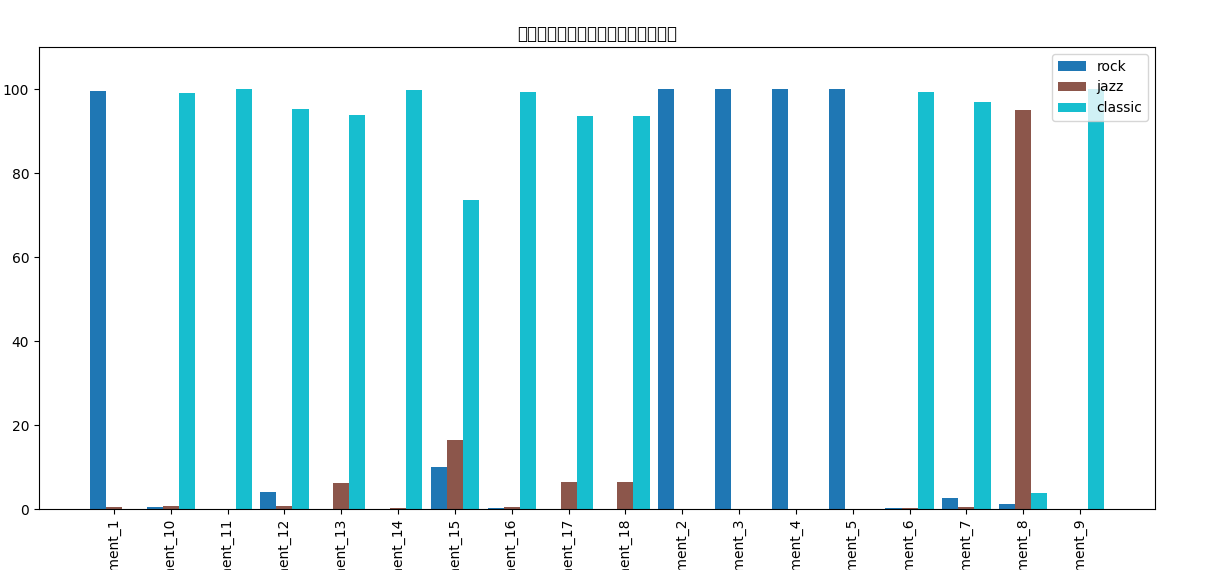
\includegraphics[width=\hsize]{fig/fig24-examhist.png}
	\caption{可視化グラフの例}
	\label{fig:examhist}
\end{figure}



\section{検証}
入力する楽曲はSnowManの「EMPIRE」\cite{EMPIRE}冒頭1分19秒を使用する．

この楽曲はモーツァルト作曲「交響曲第25番ト短調K.183」の第一楽章を\red{引用}した楽曲であり，イントロと呼ばれる冒頭部分では，\red{再び第一主題}が流れ，その後ロック調のメロディで構成される．
また，間奏部分においても\red{再び第一主題}が流れており，classicとjazzの要素が時間\red{推移}に伴い混在する楽曲となっている．
このように本楽曲は時間遷移に伴いジャンルが変化しているため，システムの検証に適していると考えた．

実際の楽器構成と本システムで抽出された楽器構成の比較を\tabref{tab:instrument2}に示す．
赤\red{色で示した}楽器は，\red{音源では}使用されているが，本システムで抽出がされなかった楽器である．
青\red{色の}楽器は，\red{音源には含まれていないにもかかわらず}本システムで抽出された楽器である．

\begin{table*}[tb]
	\centering
	\caption{実際の楽器構成と本システムで抽出された楽器構成}
	\scriptsize
	\begin{tabular}{|c|c|} \hline
		セグメント名 & 実際の楽器構成 \\ \hline\hline
		segment1  & synth, violin, \red{viola}, cello, \blue{bass} \\ \hline
		segment2  & synth, vocal, violin, \red{viola}, cello, drum \\ \hline
		segment3  & synth, vocal, violin, \red{viola}, cello, \red{oboe}, horn, drum \\ \hline
		segment4  & synth, vocal, violin, \red{viola}, cello, \red{oboe}, horn, drum, \blue{bass} \\ \hline
		segment5  & synth, vocal, \red{backing vocal}, drum \\ \hline
		segment6  & synth, vocal, \red{backing vocal}, drum, bass \\ \hline
		segment7  & synth, vocal, \red{backing vocal}, drum, bass \\ \hline
		segment8  & synth, vocal, \red{backing vocal}, drum, bass \\ \hline
		segment9  & synth, vocal, violin, \red{viola}, cello, \red{backing vocal}, drum, bas \\ \hline
		segment10 & synth, vocal, \red{backing vocal}, drum, bass \\ \hline
		segment11 & synth, vocal, \red{backing vocal}, drum, bass \\ \hline
		segment12 & synth, vocal, \red{backing vocal}, drum, bass \\ \hline
		segment13 & synth, vocal, \red{backing vocal}, drum, bass \\ \hline
		segment14 & vocal, violin, \red{viola}, cello, \red{backing vocal}, drum, bass \\ \hline
		segment15 & vocal, violin, \red{viola}, cello, \red{backing vocal}, drum, bass \\ \hline
		segment16 & synth, vocal, violin, \red{viola}, cello, \red{backing vocal}, drum, \blue{bass} \\ \hline
		segment17 & synth, vocal, violin, \red{viola}, cello, \red{oboe}, horn, \red{backing vocal}, drum, bass \\ \hline
		segment18 & vocal, violin, \red{viola}, cello, \red{oboe}, horn, \red{backing vocal}, drum, bas \\ \hline
		segment19 & synth, vocal, violin, \red{viola}, cello, \red{oboe}, horn, \red{backing vocal}, drum, bass \\ \hline
		segment20 & synth, vocal, violin, \red{viola}, cello, \red{oboe}, horn, \red{backing vocal}, drum, bass \\ \hline
		segment21 & synth, vocal, violin, \red{viola}, cello, \red{oboe}, horn, \red{backing vocal}, drum, bass \\ \hline
		segment22 & synth, vocal, violin, \red{viola}, cello, \red{oboe}, horn, \red{backing vocal}, drum, bass \\ \hline
		segment23 & synth, vocal, violin, \red{viola}, cello, \red{oboe}, horn, \red{backing vocal}, drum, bass \\ \hline
		segment24 & synth, vocal, violin, \red{viola}, cello, \red{oboe}, horn, \red{backing vocal}, drum, bass \\ \hline
		segment25 & synth, vocal, violin, \red{viola}, cello, \red{oboe}, horn, \red{backing vocal}, drum, bass \\ \hline
		segment26 & synth, vocal, violin, \red{viola}, cello, \red{oboe}, horn, \red{backing vocal}, drum, bass \\ \hline
		segment27 & synth, vocal, violin, \red{viola}, cello, \red{oboe}, horn, \red{backing vocal}, drum, bass \\ \hline
	\end{tabular}
	\label{tab:instrument2}
\end{table*}

使用した分類モデルは'voice'や'vocal'といった分類は出来るが，'backing vocal'を抽出することは困難であった．
そのため，実際は'vocal'が使用されているセグメントのほとんどで'backing vocal'も使用されているが，抽出された楽器構成では'backing vocal'が検出されていないという結果となった．
'backing vocal'の抽出が困難な理由として，'backing vocal'の音色は声楽であり，PPANsでは'vocal'と区別することが出来ないためだと考えられる．

しかし，データベースを見ると'backing vocal'は，'vocal'が使用されている楽曲のほとんどで使用されている．
そのため，自音楽ジャンルの一致率を算出するうえで重要な要素とならないと考える．

また，今回の結果から'oboe'や'viola'といった音響特徴の識別が困難な楽器は，抽出することが困難であると考えられる．
さらに，いくつかのセグメントで'bass'が誤認識されている．
その他の楽器に関しては高い楽器抽出精度といえる．

次に，音楽ジャンル\red{の一致率}を\figref{fig:EMPIREs}に示す．

抽出された楽器構成リストから，segment1からsegment4，segment7，segment9，segment10，segment14からsegment27は，弦楽器である'violin'と'cello'が含まれている．
弦楽器はデータベースの中でclassicに多く使用されており，classicの音楽ジャンル一致率が高くなると考えられる．
この箇所は楽曲中のイントロと呼ばれる冒頭部分とサビの部分であり、サンプリング元の楽曲が流れている箇所である。
このことからもclassicの音楽ジャンル一致率が高くなることが適切であるといえる。

また，segment3，segment4，segment9，segment14からsegment27には'horn'が含まれている．
'horn'は，データベースの中でclassicのみに使用されている楽器であり，このことからclassicであることを決定づける重要な要素であると考えられる．
そのためこれらのセグメントは，classicの音楽ジャンル一致率がもっとも高くなるセグメントであると考えられる．

出力されたグラフは，この考察と一致しており，音楽ジャンルの一致率計算方法は適切であるといえる．

\begin{figure}[tb]
	\centering
	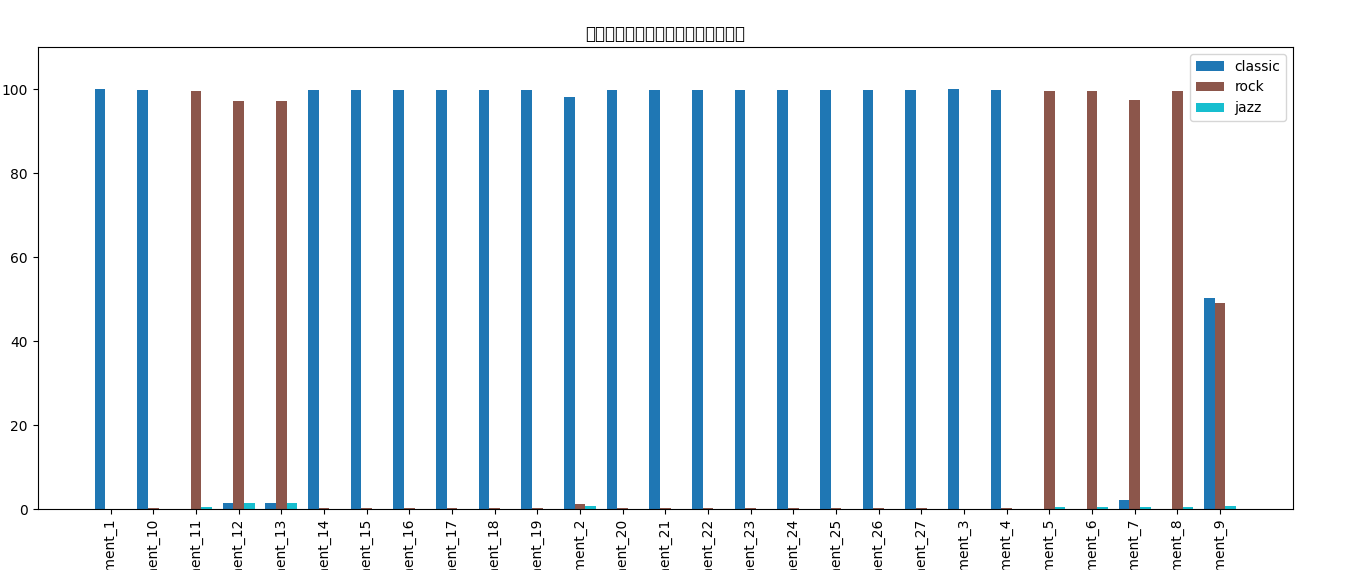
\includegraphics[width=\hsize]{fig/fig36-EMPIREs.png}
	\caption{EMPIREの音楽ジャンル一致率可視化グラフ}
	\label{fig:EMPIREs}
\end{figure}


\section{今後の課題}
今回は\red{50曲$\times$3ジャンルの}150曲のデータベースを使用した．
しかし，より正確かつ汎用性の高いシステムになるために，データベースの拡大が必要であると考える．

また，本システムでは楽器構成の抽出に音響分類モデル(PANNs)を使用した．
その結果，'backing vocal'と'oboe'を抽出することが困難であった．
これは，使用した分類モデルが'vocal'と区別できないため，また，音響特徴量の識別が困難な楽器であったためと考えられる．
今回のデータベースの規模であれば音楽ジャンルの一致率算出に大きな影響は無かったが，今後データベースを拡大していくにあたって影響が出てくる可能性がある．
そのため，より高精度な機械学習モデルを使用するなど，楽器抽出の改善も今後の課題であると考える．


\section{おわりに}
本研究では，楽曲中の時間推移に伴う音楽ジャンルの変化を分析・可視化するシステムを提案し，検証を行った．
従来の研究である1つの楽曲を1つの音楽ジャンルに分類する解析手法では捉えきれなかったジャンルの多様性に注目し，楽器構成の変化を時間軸に沿って解析することで，楽曲内でジャンルがどのように移り変わるかを可視化する新しいアプローチを示した．

提案システムでは，分割した入力音声データをPANNsを用いて楽器推定を行ったうえで，抽出された楽器構成をデータベースと照合して各ジャンルの一致率を計算し，楽曲内のジャンル変遷を可視化することが可能となった．

システム検証の結果時間経過に伴うジャンルの変化が明確に示され，本システムが音楽ジャンルの動的分析に有効であることが確認された．
一方で、'backing vocal' や 'oboe' など一部の楽器の識別が困難である課題も見られた．

今後の課題として，データベースの拡充によるジャンル分析の精度向上や，より高性能な機械学習モデルの適用により楽器抽出の精度向上があげられる．
また，ユーザビリティの向上を図るためのインターフェース改良も検討すべき点である．

本研究は，音楽ジャンル解析における新たな視点を提供し，音楽の多様性を捉える手法の一端を示した．
本システムが音楽理解の深化や楽しみ方の多様化に寄与することを期待する．


\begin{acknowledgment}
	本稿の執筆にあたり，指導教員である橋田光代准教授には多くのご指導をくださった．
	心から深謝する．
\end{acknowledgment}

